\chapter{I termin 2010 - odsłona 1 i 2}
%%%%%%%%%%%%%%%%%%%%%%%%%%
\section{zadanie 1}
\begin{framed}
Przedstaw ideę algorytmu Boruvki (Sollina).
\end{framed}
$G$ - nasz graf
$G'$ - nasza odpowiedź, początkowo tylko wierzchołki z $G$ i żadnych krawędzi
Wykonujemy kroki:
\begin{enumerate}
\item Dla każdego wierzchołka w $G$ znajdź najkrótszą incydentną krawędź i dodaj ją do $G'$
\item Utwórz nowy graf $G'$, w którym wierzchołkami są spójne składowe w starym $G'$
 \end{enumerate}
Iterujemy do póki nie zostanie jednen wierzchołek. Wszystkie dodane krawędzie do $G'$ utworzą odpowiedź.
%%%%%%%%%%%%%%%%%%%%%%%%%%%
\section{zadanie 2}
\begin{framed}
Które z poniższych algorytmów mogą działać niepoprawnie dla grafów z ujemnymi wagami krawędzi? Odpowiedź uzasadnij.
\begin{enumerate}[a)]
	\item algorytm Kruskala
	\item algorytm Prima
	\item algorytm Dijsktry
\end{enumerate}
\end{framed}

\begin{enumerate}[a)]
\item Kruskala - działa dobrze
\item Prima - działa dobrze
\item Dijkstra - Jeżeli gdzieś w grafie występuje cykl o negatywnej wadze, to wszystkie drogi nie mają najkrótszej ścieżki. Algorytm może tego nie wykryć, bo nigdy nie wraca do wierzchołków już rozważonych, a cykl możemy znaleść dopiero pod koniec wykonania, dlatego zwróci jakieś wartości dla wierzchołków, a nie powinien.
\end{enumerate}

%%%%%%%%%%%%%%%%%%%%%%%%%%%
\section{zadanie 3}
\begin{framed}
 Rozważmy następujące kryterium zrównoważenia drzew:
$$ l(w) < \alpha l(v) $$
dla każdego wierzchołka $v$ i dla każdego jego syna $w$, gdzie $l(v)$ oznacza liczbę liści w poddrzewie o korzeniu w $v$ a $\alpha$ jest pewną liczbą mniejszą od 1.
Czy ten warunek gwarantuje, że w drzewie nie powstaną długie ścieżki?
\end{framed}
TODO Przy założeniu, że $\alpha$ jest różna, dla każdego miejsca.

  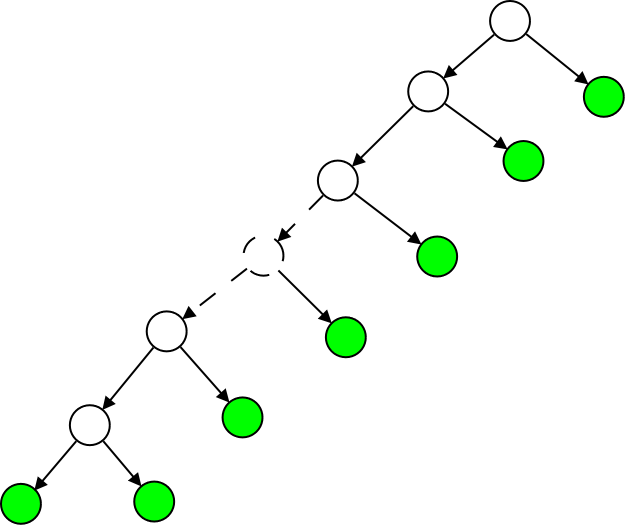
\includegraphics[width=10cm]{images/3.png}
  
Zielone to liście.
Jeżeli skonstruujemy drzewo w taki sposób, jak na rysunku, to widzimy, zę w każdym punkcie niezmiennik jest spiełniony.
W każdym wierzchołku, który ma synów, dokonujemy podziału pozostałych elementów w stosunku $(k-1):1$.

Ścieżka jest liniowej długości, bo ma długość około $0.5n = O(n)$, czyli jest długa.

%%%%%%%%%%%%%%%%%%%%%%%%%%%
\section{zadanie 4}
\begin{framed}
O ile co najwyżej może zwiększyć się liczba drzew w kopcu Fibonacciego w skutek wykonania  pojedynczej operacji $decreasekey$?
\end{framed}
Zmniejszamy wartość liścia znajdującego się na najniższym poziomie w największym drzewie w kopcu. Jeśli wszyscy przodkowie tego liścia mają po jednym synu(czyli są zaznaczone jak mówi CLRS), wtedy kaskadowo odcinamy każdego przodka liścia, tworząc nowe drzewo w kopcu.
Czyli liczba drzew zwiększy się o wysokość największego drzewa w kopcu.
Ta liczba wynosi $k = O(\log n)$, bo wiemy, że drzewo o stopniu $k$ ma wykładniczą ilość elementów, może być to jedyne drzewo, więc $n=2^k$.

%%%%%%%%%%%%%%%%%%%%%%%%%%%
\section{zadanie 5}
\begin{framed}
Dla której z podanych struktur danych koszt (najgorszego przypadku) wykonania operacji $find(i)$ sprawdzającej czy klucz $i$ jest pamiętany w strukturze jest $O(\log n)$, gdzie $n$ jest rozmiarem struktury?
\begin{enumerate}[a)]
	\item drzewo binarnych przeszukiwań
	\item drzewo AVL
	\item kopiec
	\item kopiec dwumianowy
	\item kopiec Fibonacciego
	\item drzewo czerwono-czarne
\end{enumerate}
\end{framed}
\begin{enumerate}[a)]
\item drzewo poszukiwań binarnych - może być listą - $O(n)$
\item drzewo AVL - niezmienniki gwarantuja zrównoważenie - $O(\log n)$
\item kopiec -  w ogóle nie ma posortowania - $O(n)$
\item kopiec dwumianowy - j.w. - $O(n)$
\item drzewa czerwono-czarne - jak AVL - $O(\log n)$
\end{enumerate}

 %%%%%%%%%%%%%%%%%%%%%%%%%%%
\section{zadanie 6}
\begin{framed}
Rozwiąż równanie rekurencyjne
$$ T(1)=1$$
$$ T(2)=3$$
$$ T(n)=T(n-2)+2n-1 \qquad \mbox{ dla $n >2$} $$
\end{framed}
$$ T(1)=1$$
$$ T(2)=3$$
$$ T(n)=T(n-2)+2n-1=T(n-2)+n+(n-1) \qquad \mbox{ dla $n >2$} $$

$$ T(n)=n+(n-1)+T(n-2)=$$
$$ = n+(n-1)+(n-2)+(n-3)+T(n-4)=$$
$$ = n+(n-1)+(n-2)+(n-3)+\cdots+4+3+2+1=$$
$$= \frac {n(n+1)} 2$$


%%%%%%%%%%%%%%%%%%%%%%%%%%%
\section{zadanie 7}
\begin{framed}
Który z poniższych algorytmów sortowania może w najgorszym przypadku wykonać $\Omega(n^2)$ porównań:
\begin{enumerate}[a)]
	\item quicksort
	\item mergesort
	\item insertsort
\end{enumerate}
Przypomnienie: $\Omega(n^2)$ oznacza nie mniej niż $cn^2$ dla pewnej stałej $c>0$.
\end{framed}
\begin{enumerate}[a)]
	\item quicksort - jeżeli znajdowanie pivota jest źle zrobione, tzn. odcina stałą liczbę elementów przy każdym partition, np. stosunek $1:(n-1)$, to wtedy złożoność to $n*O(n) = O(n^2)$
	\item mergesort - worst case $O(n\log n)$
	\item insertsort - posortowany lub odwrotnie posortowany ciag bedzie mieć $O(n^2)$
\end{enumerate}

%%%%%%%%%%%%%%%%%%%%%%%%%%%
\section{zadanie 8}
\begin{framed}
Złożoność algorytmu magicznych piątek wyraża się nierównością
$$ T(n) \leq T(\lceil n/5\rceil) + T(\lceil 7n/10\rceil) + O(n) $$
Wyjaśnij skąd biorą się składniki po prawej stronie nierówności. Uzasadnij czemu $T(n)$ jest $\theta(n)$.
\end{framed}
\begin{itemize}
\item $T(\lceil n/5\rceil)$ - podczas algorytmu dzielimy elementy na piątki, w każdej piątce znajdujemy medianę i rekurencyjnie wybieramy medianę z tych $\lceil n/5 \rceil$ median, aż zostanie jedna wartość.
\item $T(\lceil 7n/10\rceil)$ - jak znaleźliśmy już medianę median z kroku wyżej, to wiemy z przechodniości mniejszości, że ten element jest większy od, co najmniej, $3n/10$ elementów (w każdej piątce mediana była większa od 2 elementów, my bierzemy medianę median, czyli w połowie piątek nasz element był większy od 3 elementów).
\item $O(n)$ - koszt przejścia przez elementy i znalezienia median piątek.
\end{itemize}
\textbf{Dlaczego jest $\theta(n)$}
$$T(n) \leq T(1n/5)+T(7n/10)+O(n)= c(4n/20 + 14n/20)+O(n)= cn - (2n/20 - O(n)) \leq cn$$

Dobieramy $c$ na tyle duże, żeby pasowało do wartości kosztu obu wywołań.

%%%%%%%%%%%%%%%%%%%%%%%%%%%
\section{zadanie 9}
\begin{framed}
Napisz procedurę partition (nie musi być to wersja z wykładu, ale musi być efektywna).
\end{framed}
Pivot jest w A[p], funkcja zwaraca granicę podziału
\begin{lstlisting}
Part(A[1..n], p, r)
  x <- A[p] 
  i <- p-1 
  j <- r+1
  
   while(i<j) do
     repeat(j--) until A[j] <= x
     repeat(i++) until A[i] >= x
    
     if(i<j) swap(A[i], A[i])
     else return j 
\end{lstlisting}

%%%%%%%%%%%%%%%%%%%%%%%%%%%
\section{zadanie 10}
\begin{framed}
Narysuj drzewo binarnych wyszukiwań pamiętające klucze 1,2,3,4,5, które
\begin{enumerate}[a)]
	\item jest drzewem AVL
	\item nie jest drzewem AVL
\end{enumerate}
\end{framed}

  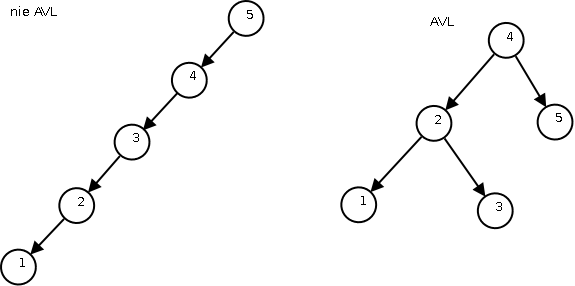
\includegraphics[width=16cm]{images/10.png}

%%%%%%%%%%%%%%%%%%%%%%%%%%%
\section{zadanie 11}
\begin{framed}
Przedstaw strategię zachłanną algorytmu aproksymacyjnego dla problemu Set Cover o współczynniku aproksymacji $H_n$.
\end{framed}
Problem: Wybrać najmniejszy taki podzbiór z rodziny zbiorów, aby wszystkie pojedyncze elementy z całej rodziny znalazły sie w tym podzbiorze.
Algorytm aproksymacyjny: W każdym kroku odrzucamy zbiór, który nie pokrywa jak nawiekszej części elementów.
\begin{lstlisting}
U - uniwersum do pokrycia
R - wejsciowa rodzina zbiorow
W - wynikowa rodzina zbiorow na poczatu pusta

while U jest niepusty
    wybierz takie Z z R ze Z przekroj U jest maksymalne
    dodaj Z do rodziny wynikowej W
    U \= Z
    usun Z z R
\end{lstlisting}

%%%%%%%%%%%%%%%%%%%%%%%%%%%
\section{zadanie 12}
\begin{framed}
Ile operacji $join$ wykona się podczas łączenia kopców dwumianowych (wersja eager) zawierających odpowiednio 53 i 35 elementów.
Przypomnienie: operacja $join$ łączy dwa drzewa dwumianowe tego samego rzędu.
\end{framed}

Tyle ile jest binarnych carry podczas dodawania 35 i 53.\\
0100011\\
0110101\\
——-\\
1011000

Wychodzi 4.

%%%%%%%%%%%%%%%%%%%%%%%%%%%
\section{zadanie 13}
\begin{framed}
Podaj definicję uniwersalnej rodziny funkcji hashujących.
\end{framed}

Niech $H$ będzie rodziną funkcji hashujących z $U$ w $\{0,...,m-1\}$.\\ Rodzinę H nazywamy uniwersalną, jeśli $\forall_{x,y\in U ;x\neq y} |{h \in H : h(x)=h(y)}|= \frac {|H|} m$
 
%%%%%%%%%%%%%%%%%%%%%%%%%%%
\section{zadanie 14}
\begin{framed}
Ile różnych dzewców można utworzyć dla n-elementowego zbioru kluczy $\{ a_1, \ldots , a_n \}$, którego pewnym dwóm elementom omyłkowo przypisano takie same priorytety (a pozostałym różne)?
\end{framed}

Wiemy, że dla jednego setu priorytetów i kluczy mamy jednego możliwego drzewca. Zakładamy raz, że jeden z równych priorytetów jest wyższy - mamy 1. drzewca, potem zakładamy, że jest niższy - mamy 2. drzewca.
%%%%%%%%%%%%%%%%%%%%%%%%%%%
\section{zadanie 15}
\begin{framed}
Na czym polega opracja kaskadowego odcinania w kopcach Fibonacciego?
\end{framed}

Żeby zachować niezmienniki potrzebne do amortyzowanej złożoności, nie pozwalamy w operacji odcięcia, usunięcia więcej niż jednego poddrzewa z jednego wierzchołka.
Dlatego zaznaczamy ojca, który utracił jednego syna i przy próbie usunięcia mu kolejnego syna usuwamy całe poddrzewo i dodajemy je do ogólnej listy.
Po tym markujemy jego dziadka (jeżeli jest zmarkowany, to znowu usuwamy poddrzewo i rekurencyjnie w gore).

%%%%%%%%%%%%%%%%%%%%%%%%%%%
\section{zadanie 16}
\begin{framed}
Ile drzew może zawierać n-elementowy kopiec dwumianowy (w wersji lazy) po wykonaniu operacji deletemin?
\end{framed}

Mamy n-elementowy kopiec w wersji lazy. Robimy deletemin. W najgorszym przypadku minimum będzie w korzeniu największego drzewa w kopcu.
 Wysokość tego drzewa to $ k = {\lfloor log_2{n}\rfloor} + 1$.\\
 Wielkość tego drzewa to oczywiście $2^{\lfloor log_2{n}\rfloor}$.\\
 Wiadomo też z definicji drzewa dwumianowego, że drzewo wysokości $k$ posiada $k-1$ synów, z których każdy jest korzeniem drzewa wysokości kolejno $k-1,k-2,..., 1$.
 Zatem usuwając minimum z drzewa o wysokości $k$ dodajemy do kopca $k-1 = \lfloor log_2{n}\rfloor$ nowych drzew.
 
%%%%%%%%%%%%%%%%%%%%%%%%%%%
\section{zadanie 17}
\begin{framed}
W algorytmie czterech Rosjan obliczane są iloczyny macierzy o rozmiarze $ n x \log n$ i macierzy o rozmiarze $ \log n x n$ Ile takich iloczynów jest obliczanych?
\end{framed}

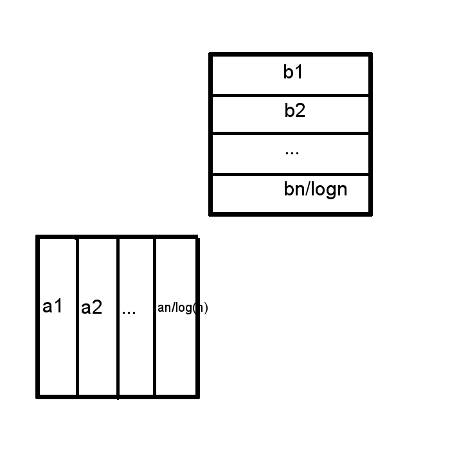
\includegraphics[scale=0.55]{images/17.png}

Liczymy iloczyny macierzy dla każdego $a_i \cdot b_i$. Takich iloczynów jest oczywiscie $\frac{n}{\log(n)}$, 
a każdy w wyniku daje jedną macierz kwadratową. Jeśli zsumujemy te macierze to otrzymamy iloczyn, o który nam chodzi.

%%%%%%%%%%%%%%%%%%%%%%%%%%%
\section{zadanie 18}
\begin{framed}
Opisz, w jaki sposób DFS może być zastosowane do znalezienia cyklu Eulera w grafie.
\end{framed}

Graf przechodzimy przy pomocy rekurencyjnej procedury DFS. Przebyte krawędzie usuwamy, a wierzchołki po zakończeniu przetwarzania umieszczamy na początku kolejki. Jeśli graf posiada cykl Eulera, to po zakończeniu algorytmu w kolejce znajdą się kolejne wierzchołki tego cyklu.

%%%%%%%%%%%%%%%%%%%%%%%%%%%
\section{zadanie 19}
\begin{framed}
Ile funkcji hashujących musimy znaleźć knstruując słownik statyczny dla zbioru n kluczy ( chodzi o konstrukcję opartą na hashowaniu dwupoziomowym).
\end{framed}

$n$ kluczy rozrzucamy do $m$ różnych tablic jedną funkcją hashującą. Potem w każdej z $m$ tablicy hashujemy elementy zamiast tworzyć listę elementów.
Czyli potrzeba $m+1$ funkcji hashujących.

%%%%%%%%%%%%%%%%%%%%%%%%%%%
\section{zadanie 20}
\begin{framed}
Narysuj sieć półczyszczacą o ośmiu wejściach.
\end{framed}

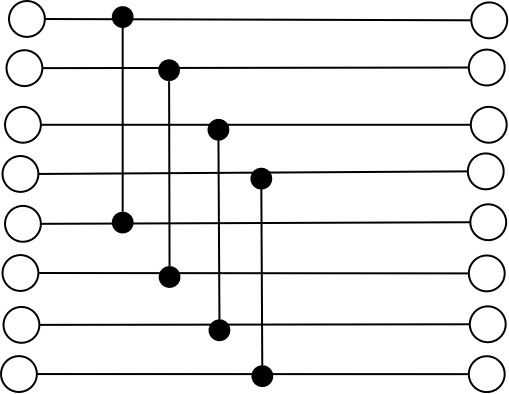
\includegraphics[scale=0.55]{images/20.png}

%%%%%%%%%%%%%%%%%%%%%%%%%%%
\section{zadanie 21}
\begin{framed}
Wylicz funkcję $\pi$ dla wzorca $abracadabra$.
\end{framed}
\begin{lstlisting}
a b r a k a d a b r a
0 0 0 1 0 1 0 1 2 3 4
\end{lstlisting}

%%%%%%%%%%%%%%%%%%%%%%%%%%%
\section{zadanie 22}
\begin{framed}
Narysuj automat rozpoznający $abaa$ i $abab$.
\end{framed}

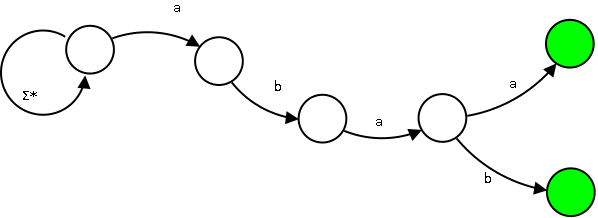
\includegraphics[scale=0.55]{images/22.png}
%%%%%%%%%%%%%%%%%%%%%%%%%%%
\section{zadanie 23}
\begin{framed}
Jaki byłby koszt wykonania ciągu $\delta$ złożonego z $O(n)$ operacji $UNION$ i $FIND$, gdyby w operacji $UNION$ zbiory były łączone w dowolny (niekoniecznie zrównoważony sposób), a operacja $FIND$ nadal byłaby wykonywana z kompresją ścieżek?
\end{framed}

Przy zastosowaniu tylko kompresji ścieżki, koszt uniona pozostaje $O(1)$, a amortyzowany koszt finda to $O(\log n)$. W najgorszym przypadku, koszt, to pewnie $O(n \log n)$.

%%%%%%%%%%%%%%%%%%%%%%%%%%%
\section{zadanie 24}
\begin{framed}
Opisz ideę algorytmu Shift-Or
\end{framed}

Niechaj T to będzie nasz tekst. m - długość wzorca W.

1. Każdej literze $\alpha$ z alfabetu przyporządkowujemy wektor $\alpha$ długości m, gdzie $\alpha[i] = 0 \Leftrightarrow W[i] = \alpha$, w przeciwnym razie 1.

2. Tworzymy wektor bitowy $V_0$ długości $m$, składający się z samych 1. Potem go SHIFTujemy i ORujemy z wektorem pierwszej literki.
Czyli $V_{0} = ( SHIFTV_0) OR S_{T[0]}$

3. Następnie robimy tak: $V_{i+1} = ( SHIFTV_i) OR S_{T[i+1]}$ - Czyli najpierw SHIFTujemy a potem ORujemy z wektorem kolejnej litery w tekście.

Dopasowanie wzorca dostaniemy gdy ostatni bit wektora $V_i$ się równa zero, czyli $V_i[m-1] = 0$

%%%%%%%%%%%%%%%%%%%%%%%%%%%
\section{zadanie 25}
\begin{framed}
W jaki sposób problem mnożenia macierzy może być wykorzystany do rozwiązania problemu najkrótszych ścieżek w grafie?
\end{framed}

Mamy grafy A i B w postaci macierzy adjacencji.\\
Możemy korzystać z algebry, w której:\\
'$+$' to działanie $\min$\\
'$\cdot$' to dodawanie\\
Wtedy jedno mnożenie macierzy, to jeden krok relaksacji najkrótszych ścieżek, musimy wykonać $n$ takich relaksacji. Złożoność $O(n^4)$. Można poprawić złożoność. Nie da się zastosować algorytmu Strassena, bo nie mamy działania odwrotnego do $\min$. Można za to skorzystać z szybkiego potęgowania, co zmniejsza nam koszt do $O(n^3\log n)$.

%%%%%%%%%%%%%%%%%%%%%%%%%%%
\section{zadanie 26}
\begin{framed}
Opisz, w jaki spósb obliczenie wielomianu n-tego stopnia w n-tych pierwiastkach jedności jest redukowalne do obliczenia dwóch wielomianów stopnia $n/2$ w $(n/2)$-tych pierwiastkach jedności.
\end{framed}

Mamy wielomian $A(x)$ stopnia $n$, reprezentowany przez współczynniki $a_0, a_1, \cdots, a_n$.\\
Tworzymy $2$ nowe wielomiany:\\
$A^{[0]}(x)=a_0 + a_2 x + a_4 x^2 + ... a_{n-2} x^{n/2 -1} + a_n x^{n/2}$\\
$A^{[1]}(x)=a_1 + a_3 x + a_5 x^2 + ... a_{n-1} x^{n/2 -1}$\\

$A(x) = A^{[0]}(x^2)+xA^{[1]}(x^2)$\\

%%%%%%%%%%%%%%%%%%%%%%%%%%%
\section{zadanie 27}
\begin{framed}
Opisz ideeę algorytmu klasy NC dla problemu dodawania dwóch liczb n-bitowych.
\end{framed}

Powiedzmy, ze mamy dodac 2 liczby n-bitowe i zalozmy ze mamy policzony wektor przeniesien:\\
$c_{n+1} c_{n} \ldots c_{3} c_{2} c_{1} c_{0}$\\
 $b_{n} \ldots b_{3} b_{2} b_{1} b_{0}$\\
+$a_{n}...a_{3} a_{2} a_{1} a_{0}$\\
wtedy wynik dodawania wyraza sie wzorem $d_i = a_i xor b_i xor c_i$\\

Teraz zobaczmy ze gdy $a_i = b_i = 0$ to $c_{i+1} = 0$ oraz gdy\\
$a_i = b_i = 1$ to $c_{i+1} = 1$ niezaleznie od tego jaki jest remainder $c_i$.\\
Ale takze gdy $a_i = 1 b_i = 0$ lub na odwrot to wtedy $c_{i+1} = c_i$.\\

Wiec zdefiniujemy sobie dzialanie * na zbiorze X = {0, 1, p}\\
dzialajace dokladnie jak powyzej czyli dla kazdego $x$ ze zbioru $X$ mamy:\\
0 * x = 0 - ustaw na 0\\
1 * x = 1 - ustaw na 1\\
p * x = x - przepisz to co masz z prawej strony\\
to dokladnie odpowiada trzem przypadkom jakie mielismy powyzej\\
dzialanie jest lacznie ale nie przemienne.\\

Teraz z wektorem przeniesien mozemy zwiazac wyrazenie:\\
czyli gdy mamy $a_i = 1 b_i = 0$ lub na odwrot to $x_i = p$ lub\\
$a_i = b_i = 1$ to $x_{i+1} = 1$ lub $a_i = b_i = 0$ to $x_{i+1} = 0$\\

Zatem z wektorem przeniesien zwiazujemy wyrazenie $x_{n+1} * x_n * ... * x_0$ gdzie $x_i \in X$ sa wyliczone jak powyzej.\\
Jesli moglibysmy policzyc wszystkie $y_i = c_i = x_i * ... * x_0$ w czasie $logn$ z uzyciem\\
wielu procesorow to mielibysmy wektor przeniesien wiec caly problem rozwiazalibysmy\\
w czasie $O(1 + logn)$.\\

Jak to policzyc jest zaprezentowane na rysunku:\\

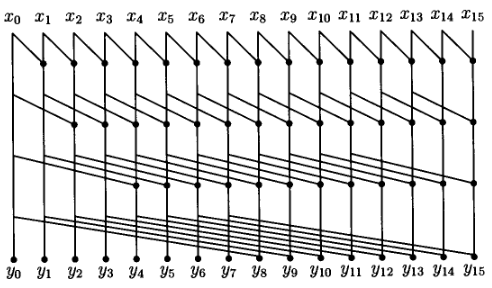
\includegraphics{images/27.png}